\documentclass[12pt,]{article}
\usepackage[utf8]{inputenc}
\usepackage[T1]{fontenc}
\usepackage{mathptmx}
\usepackage{geometry}
\usepackage{mathtools}
\usepackage[english]{babel}
\usepackage{graphicx}
\usepackage{stackengine}
\usepackage[os=win]{menukeys}
\usepackage{hyperref}
\usepackage{minted}
\usepackage{xcolor}
\usepackage{tikz}
\usepackage[yyyymmdd,hhmmss]{datetime}
\usepackage{etoolbox}
\usepackage[inline]{enumitem}

\patchcmd{\thebibliography}{\section*{\refname}}{}{}{}

\newcommand{\ShowOsVersion}{
	\immediate\write18{\unexpanded{foo=`uname -sro` && echo "${foo}" > tmp.tex}}
	\input{tmp}\immediate\write18{rm tmp.tex}
}

\newcommand{\ShowTexVersion}{
	\immediate\write18{\unexpanded{foo=`pdflatex -version | head -n1 | cut -d' ' -f1,2` && echo "${foo}" > tmp.tex}}
	\input{tmp}\immediate\write18{rm tmp.tex}
}

\addto\captionsenglish{\renewcommand{\contentsname}{Daftar Isi}}

\hypersetup{
	colorlinks=true, %set true if you want colored links
	linktoc=all,     %set to all if you want both sections and subsections linked
	linkcolor=blue,  %choose some color if you want links to stand out
	urlcolor=blue,	 %url color
}

\geometry{
	a5paper,
	left=15mm,
	right=10mm,
	top=10mm,
	bottom=15mm,
}

\title{\Large \bf
	Quick Usage Manual\\
	\small{(Mid-Testing Stage)}
}

\author{Achmadi ST MT}

\date{}

\hypersetup{citecolor=black}

\definecolor{LightGray}{gray}{0.95}

%\pagecolor[rgb]{0.1,0.1,0.1}
%\color[rgb]{1,1,1}

\begin{document}
	\maketitle
	\thispagestyle{empty}
	
	\vspace*{300pt}
	
	\noindent This manual written using: \\
	OS : \ShowOsVersion \\
	TeX : \ShowTexVersion \\
	Update: {\today} at \currenttime \\
	
	%%%%%%%%%%%%%%%%%%%%%%%%%%%%%%%%%%%%%%%%%%%%%%%%%%%%%%%%%%%%%%%%%
	
	\newpage
	\tableofcontents
	
	%%%%%%%%%%%%%%%%%%%%%%%%%%%%%%%%%%%%%%%%%%%%%%%%%%%%%%%%%%%%%%%%%
	
	\newpage
	\section{Quick Usage}
	
	\subsection{Power Up}
	
	Untuk menyalakan unit Audiometri, geser slide-switch di dekat power jack audio.
	Jika headphone telah terpasang, maka anda akan mendengar 2 tone berbunyi kanan-kiri secara bergantian
	
	\begin{figure}[!ht]
		\centering
		\includegraphics[width=350pt]{images/power_button}
		\caption{Posisi power switch}
	\end{figure}

	Sebelum memulai proses audiometri, pastikan beberapa hal berikut:
	
	\begin{itemize}
		\item Headphone sudah terpasang dan dipakai pengguna
		\item Memory Card telah terpasang.
		Jika belum, pasang MMC dan nyalakan ulang unit.
	\end{itemize}
	
	\newpage
	\subsection{Start Audiometri}
	
	Proses untuk memulai proses Audiometri
	
	\begin{figure}[!ht]
		\centering
		\includegraphics[width=350pt]{images/ledbutton_step}
		\caption{Urutan tombol dan LED interaksi proses Audiometri}
	\end{figure}
	
	Urutan untuk memulai proses audiometri adalah:
	
	\begin{enumerate}
		\item Saat kondisi \textit{idle}, LED pada posisi ini akan berkedip lambat.
		
		\item Tekan salah satu dari 3 tombol yang sebaris.
		
		\item LED terdekat dengan tombol menyala
		
		\item Tekan tombol lain selain tombol sebelumnya.
		
		\item LED sebelum nya akan mati dan LED Hijau menyala.
		Ini adalah kondisi standby/siap
		
		\item Tekan tombol lain selain dua tombol sebelumnya.
		
		\item LED pada posisi ini akan berkedip cepat dan LED lainnya akan mati.
		Proses Audiometri dimulai.
		
	\end{enumerate}
	
	Proses Audiometri akan selesai ditandai dengan LED pada langkah 1 atau 7 kembali berkedip lambat.
	
	\newpage
	\subsection{Input Audiometri}
	
	Interaksi user saat proses Audiometri pada setiap variasi frekuensi dan amplitudo secara berulang hingga proses audiometri selesai.
	
	\begin{figure}[!ht]
		\centering
		\includegraphics[width=350pt]{images/ledbutton_input}
		\caption{Urutan tombol dan LED untuk memulai}
	\end{figure}
	
	\begin{enumerate}
		\item Pastikan LED berkedip cepat sebagai indikator proses Audiometri sedang berjalan.
		
		\item Setiap LED pada grup ini akan berkedip satu kali secara berurutan.
		Salah satu diantara nya akan memberikan bunyi Tone
		
		\item Tekan satu Tombol pada grup ini sesuai LED yang menyala bersamaan dengan bunyi Tone terdengar.
		
		\item LED pada grup ini menyala salah satu. Hijau jika benar (LED, Tombol, dan Tone sesuai) dan Merah jika salah.
	\end{enumerate}

	\newpage
	\section{Formulir Survey Subyektif}
	
	Nama: ........................................\\
	
	\vspace*{20pt}
	\noindent Lingkari pilihan yang anda anggap paling cocok
	\vspace*{20pt}
	
	\noindent 1. Apakah anda sudah memahami konten manual penggunaan tersebut?\\
	\begin{itemize*}
		\item Tidak \hspace*{25pt}
		\item Kurang \hspace*{25pt}
		\item Cukup \hspace*{25pt}
		\item Lebih \hspace*{25pt}
		\item Penuh \hspace*{25pt}
	\end{itemize*}

	\vspace*{10pt}
	
	\noindent 2. Menurut anda, apakah manual tersebut menjelaskan penggunaan dengan baik?\\
	\begin{itemize*}
		\item Tidak \hspace*{25pt}
		\item Kurang \hspace*{25pt}
		\item Cukup \hspace*{25pt}
		\item Lebih \hspace*{25pt}
		\item Penuh \hspace*{25pt}
	\end{itemize*}

	\vspace*{10pt}

	\noindent 3. Menurut anda, apakah user interface (led-tombol) sudah nyaman digunakan?\\
	\begin{itemize*}
		\item Tidak \hspace*{25pt}
		\item Kurang \hspace*{25pt}
		\item Cukup \hspace*{25pt}
		\item Lebih \hspace*{25pt}
		\item Penuh \hspace*{25pt}
	\end{itemize*}

	\vspace*{10pt}
	
	\noindent 4. Menurut anda, apakah user interface (led-tombol) sudah cukup untuk proses penggunaan?\\
	\begin{itemize*}
		\item Tidak \hspace*{25pt}
		\item Kurang \hspace*{25pt}
		\item Cukup \hspace*{25pt}
		\item Lebih \hspace*{25pt}
		\item Penuh \hspace*{25pt}
	\end{itemize*}
	
	\vspace*{10pt}
	
	\noindent 5. Menurut anda, apakah dibutuhkan Display (LCD) sebagai pengganti LED indikator?\\
	\begin{itemize*}
		\item Tidak \hspace*{25pt}
		\item Kurang \hspace*{25pt}
		\item Cukup \hspace*{25pt}
		\item Lebih \hspace*{25pt}
		\item Penuh \hspace*{25pt}
	\end{itemize*}
	
	\vspace*{10pt}
	
	\noindent 6. Menurut anda, apakah dibutuhkan Touchscreen (TFT) sebagai pengganti tombol?\\
	\begin{itemize*}
		\item Tidak \hspace*{25pt}
		\item Kurang \hspace*{25pt}
		\item Cukup \hspace*{25pt}
		\item Lebih \hspace*{25pt}
		\item Penuh \hspace*{25pt}
	\end{itemize*}

	\vspace*{10pt}
	
	\noindent 7. Jika menurut anda Display LCD dibutuhkan, informasi apa yang wajib ditampilkan?\\
	...................................................................................................................................\\
	...................................................................................................................................\\
	...................................................................................................................................\\
	...................................................................................................................................\\
	...................................................................................................................................\\
	
	\noindent 8. Jika menurut anda Touchscreen dibutuhkan, informasi apa yang wajib dimasukkan?\\
	...................................................................................................................................\\
	...................................................................................................................................\\
	...................................................................................................................................\\
	...................................................................................................................................\\
	...................................................................................................................................\\
	
	\noindent 9. Menurut anda, apa yang perlu diperbaiki pada user interface yang sekarang telah tersedia?\\
	...................................................................................................................................\\
	...................................................................................................................................\\
	...................................................................................................................................\\
	...................................................................................................................................\\
	...................................................................................................................................\\
	
	\noindent 10. Menurut anda, apa yang perlu ditambahkan pada user interface untuk selanjutnya (selain Display/Touchscreen)?\\
	...................................................................................................................................\\
	...................................................................................................................................\\
	...................................................................................................................................\\
	...................................................................................................................................\\
	...................................................................................................................................\\
	
\end{document}